% Figure: Normal Tryptophan Metabolism
% Balanced split between serotonin and kynurenine pathways

\begin{figure}[htbp]
\centering
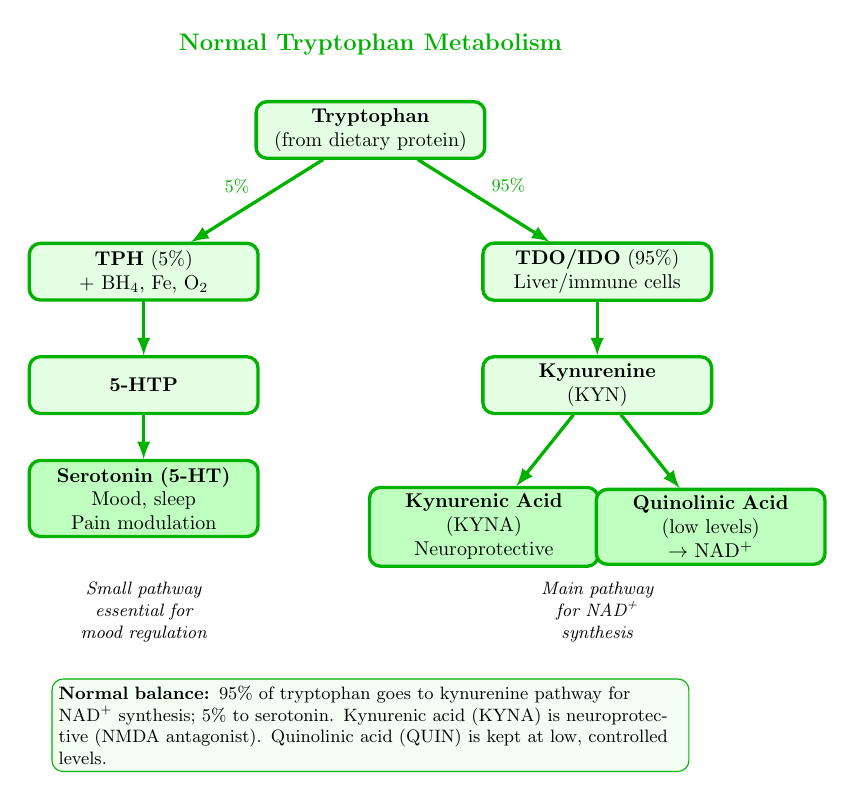
\begin{tikzpicture}[scale=0.72, every node/.style={scale=0.72},
    % Styles
    process/.style={draw=green!70!black, fill=green!10, very thick, rounded corners, text width=3.8cm, align=center, minimum height=1cm},
    output/.style={draw=green!70!black, fill=green!25, very thick, rounded corners, text width=3.8cm, align=center, minimum height=1cm},
    arrow/.style={-latex, very thick, green!70!black},
    note/.style={font=\small\itshape, text width=3cm, align=center},
]

% Title
\node[font=\large\bfseries, green!70!black] at (0, 8.5) {Normal Tryptophan Metabolism};

% Tryptophan input
\node[process] (trp) at (0, 7) {\textbf{Tryptophan}\\(from dietary protein)};

% LEFT BRANCH: Serotonin pathway (5%)
\node[process] (tph) at (-4, 4.5) {\textbf{TPH} (5\%)\\+ BH\textsubscript{4}, Fe, O\textsubscript{2}};
\draw[arrow] (trp) -- node[above left, font=\small] {5\%} (tph);

\node[process] (fivehttp) at (-4, 2.5) {\textbf{5-HTP}};
\draw[arrow] (tph) -- (fivehttp);

\node[output] (serotonin) at (-4, 0.5) {\textbf{Serotonin (5-HT)}\\Mood, sleep\\Pain modulation};
\draw[arrow] (fivehttp) -- (serotonin);

% RIGHT BRANCH: Kynurenine pathway (95%)
\node[process] (tdo) at (4, 4.5) {\textbf{TDO/IDO} (95\%)\\Liver/immune cells};
\draw[arrow] (trp) -- node[above right, font=\small] {95\%} (tdo);

\node[process] (kyn) at (4, 2.5) {\textbf{Kynurenine}\\(KYN)};
\draw[arrow] (tdo) -- (kyn);

% Kynurenine splits
\node[output] (kyna) at (2, 0) {\textbf{Kynurenic Acid}\\(KYNA)\\Neuroprotective};
\draw[arrow] (kyn) -- (kyna);

\node[output] (quin) at (6, 0) {\textbf{Quinolinic Acid}\\(low levels)\\$\rightarrow$ NAD\textsuperscript{+}};
\draw[arrow] (kyn) -- (quin);

% Notes
\node[note] at (-4, -1.5) {Small pathway\\essential for\\mood regulation};
\node[note] at (4, -1.5) {Main pathway\\for NAD\textsuperscript{+}\\synthesis};

% Key point box
\node[draw=green!70!black, fill=green!5, rounded corners, text width=11cm, align=left, font=\small] at (0, -3.5) {
\textbf{Normal balance:} 95\% of tryptophan goes to kynurenine pathway for NAD\textsuperscript{+} synthesis; 5\% to serotonin. Kynurenic acid (KYNA) is neuroprotective (NMDA antagonist). Quinolinic acid (QUIN) is kept at low, controlled levels.
};

\end{tikzpicture}
\caption{Normal tryptophan metabolism with balanced serotonin and kynurenine pathways.}
\label{fig:tryptophan-normal}
\end{figure}
